\documentclass{article}

% if you need to pass options to natbib, use, e.g.:
% \PassOptionsToPackage{numbers, compress}{natbib}
% before loading nips_2017
%
% to avoid loading the natbib package, add option nonatbib:
% \usepackage[nonatbib]{nips_2017}

\PassOptionsToPackage{numbers, compress}{natbib}
\usepackage{nips_2017}

% to compile a camera-ready version, add the [final] option, e.g.:
% \usepackage[final]{nips_2017}

\usepackage[utf8]{inputenc} % allow utf-8 input
\usepackage[T1]{fontenc}    % use 8-bit T1 fonts
\usepackage{hyperref}       % hyperlinks
\usepackage{url}            % simple URL typesetting
\usepackage{booktabs}       % professional-quality tables
\usepackage{amsfonts}       % blackboard math symbols
\usepackage{nicefrac}       % compact symbols for 1/2, etc.
\usepackage{microtype}      % microtypography

%for matrices
\usepackage{blkarray}
\usepackage{amsmath}

\usepackage{graphicx}
\usepackage{caption}
\usepackage{subcaption}

\usepackage[svgnames, table]{xcolor} % Enabling colors by their 'svgnames'

% define custom commands
\definecolor{commentPJA_color}{rgb}{1.0,0.0,0.8}
\newcommand{\commentPJA}[1]{{\textcolor{commentPJA_color}{PJA: #1}}}


% define custom commands
\definecolor{commentLP_color}{rgb}{1.0,0.0,0.8}
\newcommand{\commentLP}[1]{{\textcolor{commentLP_color}{LP: #1}}}


% define custom commands
\definecolor{commentAP_color}{rgb}{1.0,0.0,0.8}
\newcommand{\commentAP}[1]{{\textcolor{commentAP_color}{AP: #1}}}

% define custom commands
\definecolor{commentRJ_color}{rgb}{1.0,0.0,0.8}
\newcommand{\commentRJ}[1]{{\textcolor{commentRJ_color}{RJ: #1}}}


\newcommand{\mb}[1]{\mathbf{#1}}
\newcommand{\bs}[1]{\boldsymbol{#1}}
\newcommand{\mvec}[1]{\mathbf{#1}}

\title{Givens Transform Approach for Efficient Probabilistic Principle Component Analysis for Bayesian Dimensionality Reduction (GT-PPCA)}

% The \author macro works with any number of authors. There are two
% commands used to separate the names and addresses of multiple
% authors: \And and \AND.
%
% Using \And between authors leaves it to LaTeX to determine where to
% break the lines. Using \AND forces a line break at that point. So,
% if LaTeX puts 3 of 4 authors names on the first line, and the last
% on the second line, try using \AND instead of \And before the third
% author name.

\author{
  David S.~Hippocampus\thanks{Use footnote for providing further
    information about author (webpage, alternative
    address)---\emph{not} for acknowledging funding agencies.} \\
  Department of Computer Science\\
  Cranberry-Lemon University\\
  Pittsburgh, PA 15213 \\
  \texttt{hippo@cs.cranberry-lemon.edu} \\
  %% examples of more authors
  %% \And
  %% Coauthor \\
  %% Affiliation \\
  %% Address \\
  %% \texttt{email} \\
  %% \AND
  %% Coauthor \\
  %% Affiliation \\
  %% Address \\
  %% \texttt{email} \\
  %% \And
  %% Coauthor \\
  %% Affiliation \\
  %% Address \\
  %% \texttt{email} \\
  %% \And
  %% Coauthor \\
  %% Affiliation \\
  %% Address \\
  %% \texttt{email} \\
}

\begin{document}
% \nipsfinalcopy is no longer used

\maketitle

\begin{abstract}
Probabilistic PCA (PPCA) is a probabilistic generative model used for finding low dimensional representations of high-dimensional data. While PPCA is highly flexible in theory, PPCA and related models contain a constrained orthonormal matrix parameter that makes it difficult in practice to build complex PPCA-like models and conduct fully-Bayesian inference using modern algorithms like NUTS and ADVI, especially for novices. We present the geometrically-motivated Givens Transform (GT) that represents orthonormal matrices in terms of unconstrained parameters, and addresses computational issues that make PPCA-related models difficult to implement in practice. Our approach, that we refer to as GT-PPCA, allows us to rapidly build and prototype a wide range of PPCA-related models in a probabilistic programming framework like Stan, opening up the possibility for full Bayesian inference on a wide-class of models using a variety of different inference algorithms. The geometric insight provided by GT-PPCA also allows us to make useful improvements to related methods such as the reduction of superfluous multi-modality in the posterior, and new prior distributions useful for hierarchical modeling. We demonstrate these improvements and show how we use GT-PPCA in Stan (code provided) to build a hierarchical multi-view model for medical data, and a Hidden Markov Subspace Model for time-dependent disease network data.
\end{abstract}

%%%%%%%%%%%%%%%%%%%%%%%%%
\section{Introduction}
%%%%%%%%%%%%%%%%%%%%%%%%%

Probabilistic PCA (PPCA) \citep{tipping1999probabilistic} posits a probabilistic generative model where high-dimensional data is determined by a linear function of some low-dimensional latent state. This generative model readily allows us to extend PPCA to describe the generative process of our data as we see fit. For example, one can extend the standard PPCA generative process to obtain Sparse PCA \citep{hoff2009simulation}, Bayesian Exponential PCA \citep{mohamed2009bayesian}, Mixtures of Factor Analyzers \citep{ghahramani1996algorithm}, or Canonical Correlation Analysis. This flexibility is crucial for describing complex datasets arising in domains such as medicine where high-dimensional data may be stratified, consist of multiple views, or may vary over time. Despite the demonstrated flexibility of PPCA, both computational and statistical challenges that stem from orthonormal matrix parameters of PPCA stand in the way of making it a part of a routine modeling workflow. It would be ideal to be able to rapidly build and prototype diverse Bayesian linear dimensionality-reduction models in the framework of a probabilistic programming language like Stan, and subsequently infer these models using state-of-the-art inference algorithms like NUTS or ADVI that provide fully Bayesian posterior uncertainties of our estimates and prevent us from overfitting.

We draw on techniques from differential geometry and numerical analysis to introduce the Givens Transform, a novel way to represent orthonormal matrices that lets us easily build complex extensions to PPCA in Stan. We provide Stan code for our example models allowing for use and expansion by researchers and scientists out-of-the-box. We demonstrate how inference of these models in Stan yields good empirical performance on large probabilistic graphical models that were previously intractable to implement especially if fully-Bayesian posterior analysis is desired. Specifically we present a hierarchical subspace model for stratified, multi-view medical data and a PPCA Hidden Markov Model (HMM) for disease-network data.

The Givens Transform represents orthonormal matrices in terms of a sequence of fundamental rotations through given angles, yielding insight in to novel and useful ways to work with and interpret Bayesian dimensionality reduction models.  For instance, the elegant geometric representation lets us see how by limiting the range of the parameters in GT-PPCA, we can naturally avoid issues of unidentifiability and multi-modal posteriors that arise in working with orthonormal matrices.  GT-PPCA also allows us new and creative ways to generate and use prior distributions on orthonormal matrices, and thus subspaces, a task that had previously been rather complicated due to the difficulty of evaluating densities of orthonormal matrix distributions for even small problem sizes.  As we shall discuss in more detail, our GT representation provides a rather natural way to specify prior distributions comparable to the Matrix Langevin prior \citep{muirhead2009aspects}.

%When first considering this problem, it may seem that this geometry may rule out a straightforward use of two of the most prominent techniques for posterior inference posterior inference, Markov Chain Monte Carlo (MCMC) and Variational Inference (VI).  Intuitively, for MCMC, we have no way of guaranteeing that a chain over $W$ will explore only valid regions of parameter space that satisfy the orthonormality constraints. Similarly for Variational Inference, positing a common variational posterior distribution such as a Gaussian over the elements of $W$ is sure to lead to posteriors that assign mass to invalid regions of parameter space.


\paragraph{Related work} While previous authors have developed methods for posterior sampling of distributions orthonormal matrices, these methods can at times suffer from numerical issues, they are difficult to implement on large probabilistic graphical models, and they can not be used in any general inference scheme such as NUTS or VI like GT-PPCA can. \citet{brubaker2012family} and \citet{byrne2013geodesic} used separate approaches to modify the Leap-Frog integrator typically used in Hamiltonian Monte Carlo (HMC), so that Hamiltonian exploration, and thus MCMC samples of posteriors, satisfied any necessary constraints at all times. Specifically,~\citet{brubaker2012family} uses the SHAKE integrator \citep{leimkuhler2004simulating} to simulate Hamiltonian dynamics and generate proposals. The integrator works by repeatedly taking a step forward that may be off the manifold using ordinary leap frog, then projecting back down to the nearest point on the manifold. This projection is done via Newton iterations, which may converge to the wrong local minimum in practice or perhaps not converge at all, possibly jeopardizing the ergodicity of a Markov Chain, and the integrity of samples~\citep{betancourt2017divergences}. \citet{byrne2013geodesic}~took a different approach, exploiting the fact that closed form solutions are known for the geodesic equations over the Stiefel manifold in the embedded coordinates, $W$. While this method is completely explicit, requiring no Newton iterations, in practice we found that for larger step sizes, the integrator steps off the Stiefel manifold, due to the numerical imprecision of the matrix exponential function. Because these methods use modified integrators for constrained parameters, in practice they require keeping track of the support of each variable and which type of integrator to use on each variable. This adds an extra layer of implementation complexity, especially for large complex probabilistic graphical models, that makes it difficult to implement these methods within a probabilistic programming language such as Stan. This precludes the rapid prototyping and building of models as well as the flexibility to use different inference schemes that Stan provides. Lastly, we remark that for inference on orthonormal matrices, these methods can lead to multi-modal posteriors, that can be avoided in a straight-forward way using the Givens transform.

\paragraph{Paper outline} We give a brief overview of probabilistic dimensionality reduction in Section~\ref{Probabilistic dimensionality reduction}. We discuss the geometry of the Stiefel Manifold in Section~\ref{geometry}, before finally introducing the Givens Transform (GT) in Section~\ref{Givens}. Finally, we present various empirical studies where we used GT-PPCA in Stan for practical uncertainty quantification and hypothesis testing, as well as for building complex probabilistic graphical models.

%%%%%%%%%%%%%%%%%%%%%%%%%

%%%%%%%%%%%%%%%%%%%%%%%%%
%%%%%%%%%%%%%%%%%%%%%%%%%
%%%%%%%%%%%%%%%%%%%%%%%%%
\section{Probabilistic Principle Component Analysis (PPCA)} \label{Probabilistic dimensionality reduction}
%%%%%%%%%%%%%%%%%%%%%%%%%
%%%%%%%%%%%%%%%%%%%%%%%%%
%%%%%%%%%%%%%%%%%%%%%%%%%

PPCA posits the following generative process for how a sequence of high-dimensional data vectors $\mathbf{x} \in \mathbb{R}^n$ $i = 1, \cdots, N$ arise from some low dimensional latent representation $\mathbf{z} \in \mathbb{R}^p$ where $p < n$:

\begin{eqnarray}
\label{eq:PpcaGenerativeProcess}
p(\mb{z}_i) &\sim& \mathcal{N}_p(0, I) \nonumber\\
p(\mb{x}_i | \mb{z}_i, W, \Lambda, \sigma^2) &\sim& \mathcal{N}_n(W \Lambda \mb{z}_i, \sigma^2 I).
\end{eqnarray}
Here $W$ is an $n \times p$ orthonormal matrix and $\Lambda$ is a $p \times p$ diagonal matrix with positive elements.  For simplicity, we have assumed here that the data has only zero mean but the more general case can also readily be considered \citep[chapt.~12.1]{murphy2012machine}. 

\paragraph{Expanding models}
As alluded to previously, PPCA generative model can be flexibly expanded in several ways as modelers see fit. To build a probabilistic sparse PCA, one can place a Laplace or Cauchy prior over the elements of $W$. \citet{mohamed2009bayesian} showed that we can model non-Gaussian data, $\mb{x}_i$, by replacing equation \ref{eq:PpcaGenerativeProcess} with an exponential family member whose natural parameters are given by $\mathrm{Expon}(W\Lambda \mb{z}_i)$ where $\mathrm{Expon}(\cdot)$ is an appropriate link function.\citet{ghahramani1996algorithm} use a mixture of several $W$ matrices for different regions of data space to extend PPCA to the non-linear case. In Section \ref{examples}, we show such how we designate a separate $W$ parameter (subspace) for separate groups of hospital patients with different types of injuries, then place prior over these subspaces to solve a difficult transfer learning problem. In Section \ref{examples} we also extend Canonical Correlation Analysis (CCA), which is itself an extension of PPCA to multi-view data, to time-dependent multi-view data. Again, in the context of a probabilistic programming language such as Stan, these extensions to the base PPCA model become trivial to implement as we illustrate with examples in Section \ref{examples}.

\paragraph{Importance of the Orthonormality Condition}
The orthonormal constraint on the matrix $W$ plays an important role in obtaining robust methods for making inferences in probabilistic PCA because it alleviates identifiability and numerical issues.  If one were to relax the orthonormality constraint and naively conduct inference in the space of all $n\times p$ matrices, the likelihood function would assign identical probability to a whole equivalence class of matrices $W \sim V$ where the span is the same linear subspace $\mbox{span}\{W\} = \mbox{span}\{V\}$ \citet[chapt.~12.1.3]{murphy2012machine}.  Besides resulting in an unidentifiable model, in practice this presents a number of major challenges.  This first is that the matrices in a given equivalence class are not all equally well-conditioned numerically and round-off errors and truncation errors become problematic in practical calculations.  Secondly, these issues with the representation further manifest in the log-likelihood objective function where regions arise of particularly large curvature as pointed out by \citep{holbrook2016bayesian}. We note that, while most identifiability issues and numerical issues are alleviated by constraining inference to orthonormal matrices, the PPCA likelihood is equivalent for an orthonormal matrix $W$ and any permutation of the columns of $W$ being negative as pointed out by both \citet[chapt.~12.1.3]{murphy2012machine} and  \citet{holbrook2016bayesian}. As such, even the methods of \citet{brubaker2012family} and \citet{byrne2013geodesic} will lead to multi-modal posteriors, that can be avoided in a straight-forward way by appealing to insights revealed by the Givens Transform, as we explain in Section~\ref{Givens}.

%\paragraph{Inference} Inference for PPCA is typically conducted by obtaining a point estimate for $W$ via a closed-form estimator, or for expanded PPCA models via (EM) \citep[chapt.~12.2]{murphy2012machine}, neither of which provide a notion of uncertainty for our point estimates. Without information regarding the uncertainty of our estimates these point estimates could be far from the true value of $W$ and thus mislead our conclusions, especially for larger models and/or when there is relatively little data available. Furthermore, point estimates do now allow for hypothesis testing e.g. statistically testing whether two different groups of observations lie in the same subspace. We show with examples how GT-PPCA in Stan makes it easy achieve these tasks in section \ref{examples}.

%%%%%%%%%%%%%%%%%%%%%%%%%
%%%%%%%%%%%%%%%%%%%%%%%%%
%%%%%%%%%%%%%%%%%%%%%%%%%
\section{Geometry of the Stiefel Manifold} \label{geometry}
%%%%%%%%%%%%%%%%%%%%%%%%%
%%%%%%%%%%%%%%%%%%%%%%%%%
%%%%%%%%%%%%%%%%%%%%%%%%%

While specifying $W$ in Equation \ref{eq:PpcaGenerativeProcess} to be orthonormal is necessary in practice, this leaves us with having to work with prior and posterior distributions over orthonormal matrices. To make better sense of these types of objects as well as the space of orthonormal matrices we must analyze their geometric properties.

Just as three-dimensional unit vectors form a sphere in $\mathbb{R}^3$, which is a submanifold of $\mathbb{R}^3$, the set of $n\times p$ orthonormal matrices, form a sub-manifold in the space of general $n \times p$ matrices known as the Stiefel Manifold and denoted $V_{n,p}$\citep{muirhead2009aspects}. $V_{n,p}$ is formally defined as

\begin{equation}
V_{n,p} := \{Y \in \mathbb{R}^{n \times p}: YY^T = I \}.
\end{equation}

Intuitively, the elements of $V_{n,p}$ can be thought of not as orthonormal matrices, but as $p$-frames which are comprised of $p$ orthonormal vectors that lie in $n$-dimensional space. To move about the Stiefel manfiold, one can rigidly rotate the vectors in the $p$-frame about any combination of axes an arbitrary number of times. In the case where $n = 3$ and $p = 2$, this is almost identical to sphere (Figure \ref{fig:StiefelGeom}), but with an extra angle, $\theta_{23}$ that controls how much the second basis vector is rotated about the first. For a three-dimensional set of points forming a flat, pancake-like cloud, PPCA can be thought of as finding the best $2$-frame that aligns with this cloud.

\begin{figure}
    \centering
    \begin{subfigure}[b]{0.3\textwidth}
        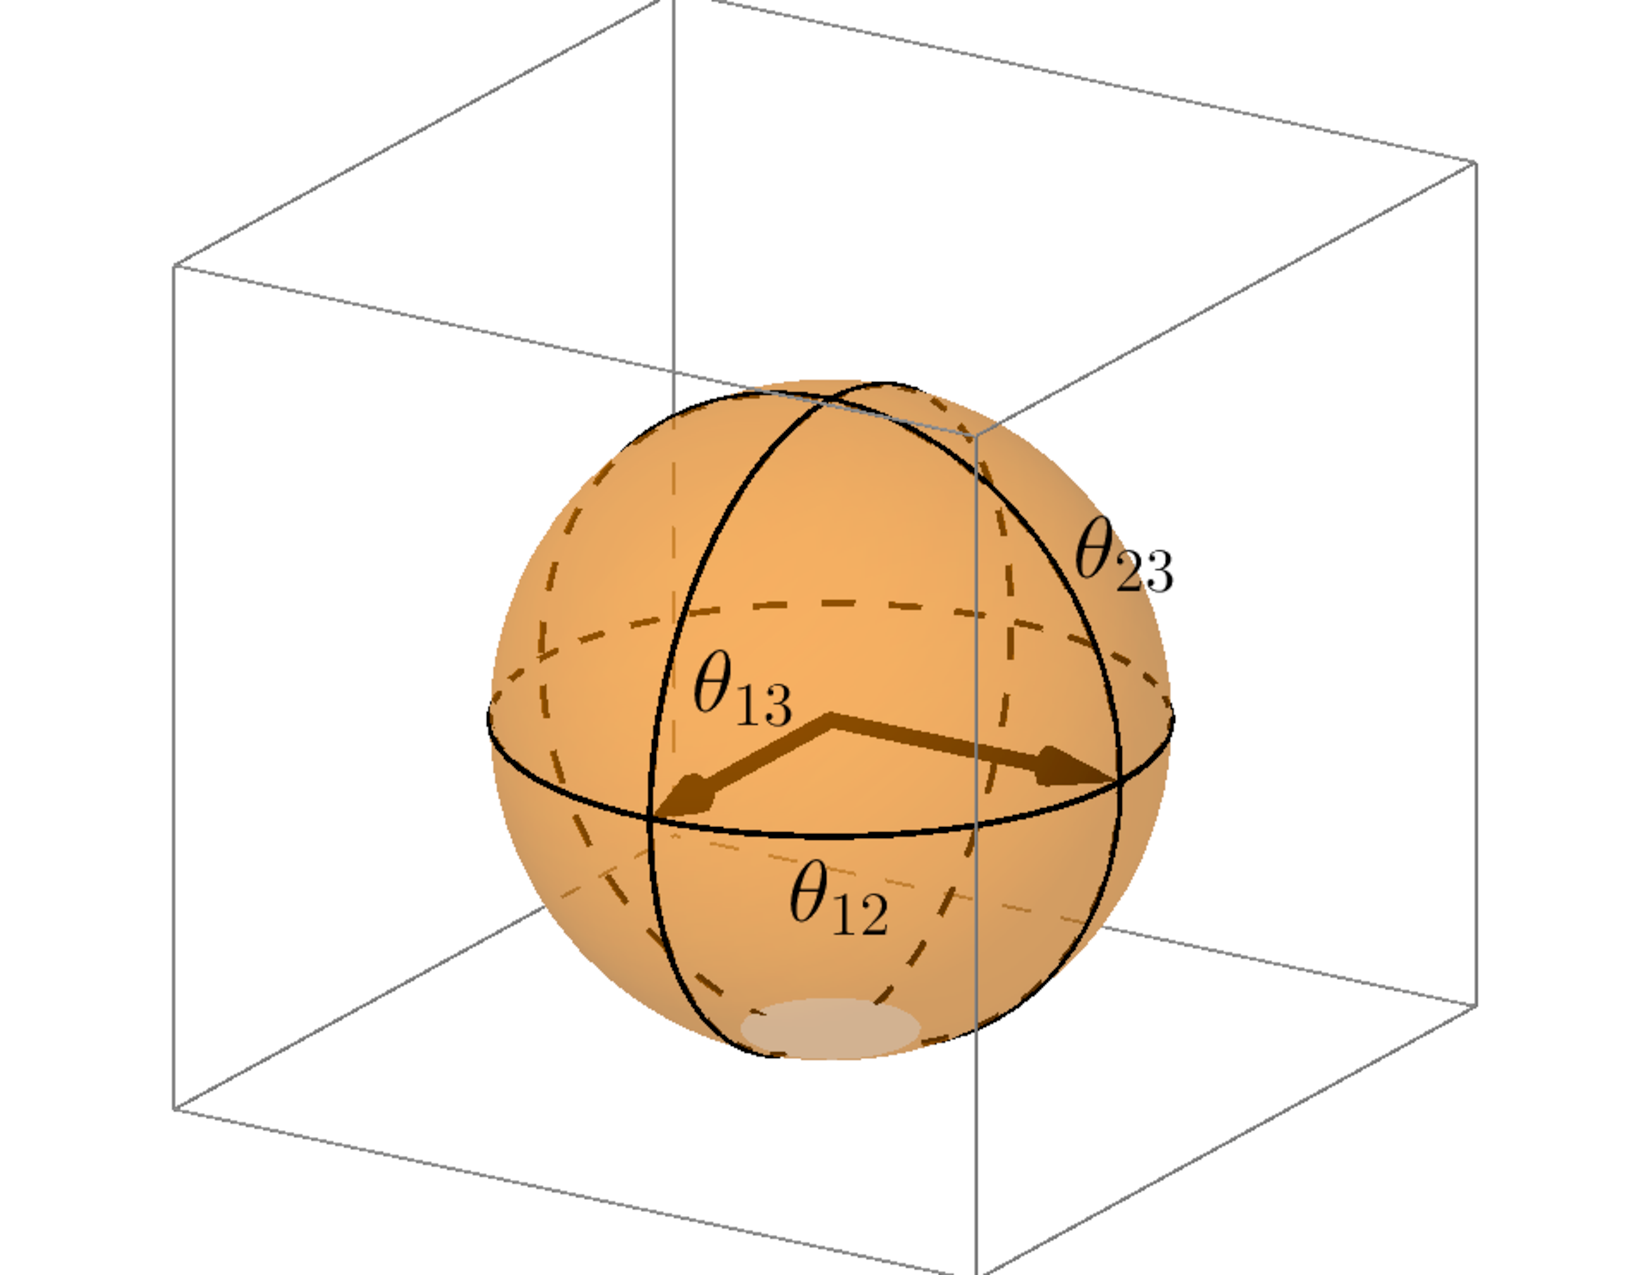
\includegraphics[width=\textwidth]{StiefelGeom.pdf}
        \caption{}
        \label{fig:StiefelGeom}
    \end{subfigure}
    ~ %add desired spacing between images, e. g. ~, \quad, \qquad, \hfill etc. 
      %(or a blank line to force the subfigure onto a new line)
    \begin{subfigure}[b]{0.3\textwidth}
        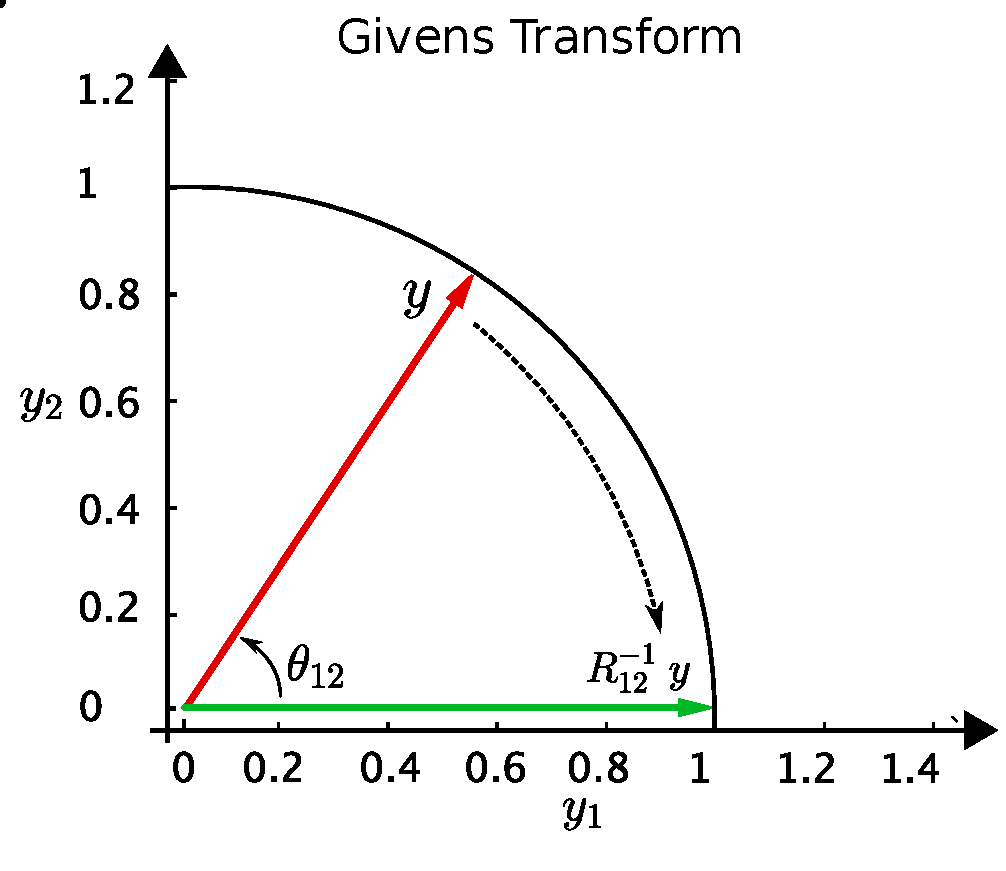
\includegraphics[width=\textwidth]{GivensReduction_atz.pdf}
        \caption{}
        \label{fig:GivensReductionm}
    \end{subfigure}
    ~ %add desired spacing between images, e. g. ~, \quad, \qquad, \hfill etc. 
    %(or a blank line to force the subfigure onto a new line)
    \begin{subfigure}[b]{0.3\textwidth}
        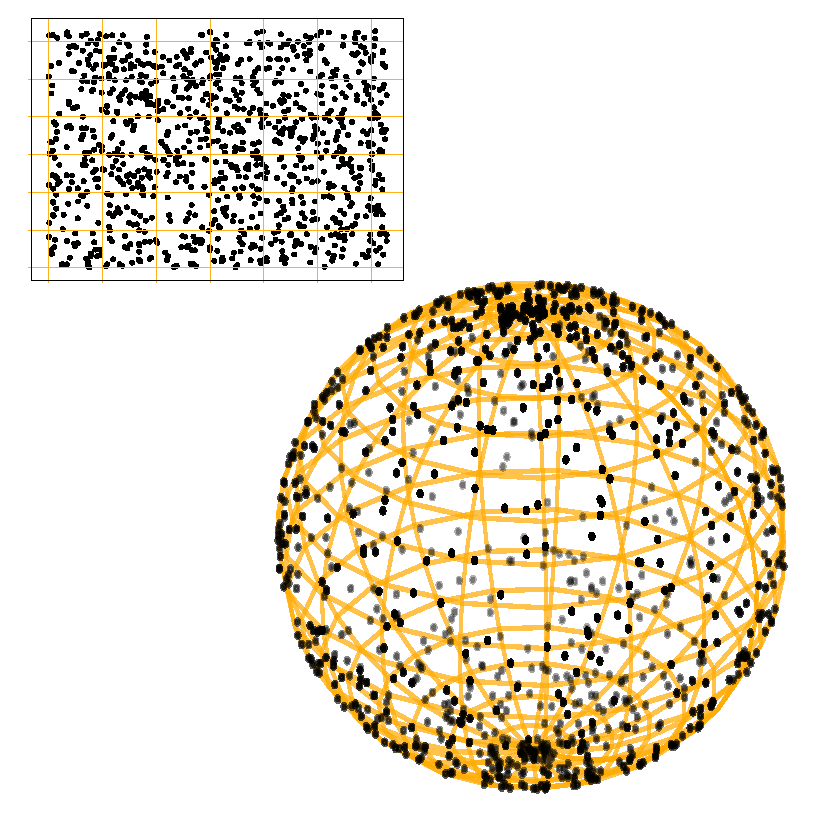
\includegraphics[width=\textwidth]{AreaForm.pdf}
        \caption{}
        \label{fig:AreaForm}
    \end{subfigure}
    \caption{Visualizing the Givens Transform. (a) How the Givens Reduction ``zeros out'' a column vector. (b) A geometric view of the Stiefel manifold, two-frame in three dimensions. (c) Sampling without a proper measure adjustment. }\label{fig:Givens}
\end{figure}
 
While $n \times p$ orthonormal matrices are represented by $np$ elements, the Stiefel Manifold $V_{n,p}$, has an intrinsic dimension of $np-p(p+1)/2$. This arises from the constraints on the columns of the matrix that impose orthonormality.  This dimensionality can be seen by observing, that the first column of $Y \in V_{n,p}$ must have norm one and hence has one constraint placed on it. The second column must also have norm one and also must be orthogonal to the first column hence with two constraints placed on it.  Continuing to the third column through the $n^{th}$ one arrives at the conclusion that each point of the Stiefel Manifold has only $np - (1+2+\cdots+p) =np-p(p+1)/2$ degrees of freedom.  The Givens transform can be thought of as an $np-p(p+1)/2$-dimensional set of coordinates $\Theta$, that represent elements of the Stiefel manifold.

%%%%%%%%%%%%%%%%%%%%%%%%%
%%%%%%%%%%%%%%%%%%%%%%%%%
%%%%%%%%%%%%%%%%%%%%%%%%%
\section{Givens Transform (GT) approach to PPCA (GT-PPCA)} \label{Givens}
%%%%%%%%%%%%%%%%%%%%%%%%%
%%%%%%%%%%%%%%%%%%%%%%%%%
%%%%%%%%%%%%%%%%%%%%%%%%%

%\paragraph{Transformed random variables} Posterior distributions for constrained parameters in probabilistic graphical models are routinely inferred by transforming such parameters to an unconstrained space and seeking posterior distributions over the transformed parameter~\citep{carpenter2016stan, kucukelbir2014fully}. This requires a smooth one-to-one transformation $f: \mathrm{supp}(z_\mathrm{constr}) \to \mathbb{R}^D$, where $\mathrm{supp}(z_\mathrm{constr})$ is the support of the constrained random variable $z_\mathrm{constr}$. To our knowledge, no such transformation has been proposed to map orthonormal matrices to a comparable unconstrained space.

Posterior distributions for several types of constrained parameters are routinely inferred in practice using both MCMC and VI by transforming the constrained variables to an unconstrained space. Using a one-to-one mapping $T: \mathrm{supp}(z_\mathrm{constr}) \to \mathbb{R}^D$, where $\mathrm{supp}(z_\mathrm{constr})$ is the support of the constrained random variable $z_\mathrm{constr}$,and $T$ is a smooth one-to-one transformation, one can obtain a posterior over the unconstrained parameter that corresponds to the original constrained parameter of interest, then map inferences back to the original constrained space. This procedure requires computing the Jacobian, $J_{T^{-1}}$ of the transformation, to obtain $f_{Y}(y) = f_{z_\mathrm{constr}}(T^{-1}(y)) J_{T^{-1}}(y)$ where $Y$ is an unconstrained random variable with probability density function (PDF) $f_Y$ and $f_{z_\mathrm{constr}}$ is the probability density of $z_\mathrm{constr}$, which for PPCA comes from equation \ref{eq:PpcaGenerativeProcess}. The extra Jacobian term accounts for how the a unit volume under the transformation changes \citep{kucukelbir2014fully}. Without this extra Jacobian factor, inference between the two spaces is incomparable. For example, uniformly sampling in spherical coordinates (unconstrained space) does not correspond to uniformly sampling on the sphere (constrained space), unless we include an appropriate term accounting for how volumes are warped under the transformation (see Figure \ref{fig:AreaForm}). Intuitively, ares that are near the poles get shrunk far more than areas near the equator, so when mapped back on to the sphere, points will congregate closer to the poles of the sphere. Conducting inference in a transformed space is most notably used in ADVI and Stan's HMC routines \citep{carpenter2016stan, kucukelbir2014fully}. To our knowledge no such transform, other than the Givens Transform we introduce next, has been proposed for orthonormal matrices. In sub-section \ref{GivensSub} we briefly discuss Givens Reductions which motivate and lead into our explanation of the Givens Transform. In sub-section \ref{geomGivens} we discuss geometric aspects of the Givens transform such as avoiding multi-modality and including a term that measures how volume is changed under the transform that is analogous to the Jacobian described above. 

%%%%%%%%%%%%%%%%%%%%%%%%%
\subsection{Givens Reductions and the Givens Transform}\label{GivensSub}
%%%%%%%%%%%%%%%%%%%%%%%%%
The Givens Reduction is a numerical analysis technique for reducing a square matrix $A$ to upper-triangular form \citep{meyer2000matrix}. The technique works by applying a series of rotation of matrices to $A$ such that elements below the diagonal are ``zeroed out" starting with the second element of the first column, and moving down the first column before zeroing out the appropriate elemnents of the subsequent columns. For example if $A$ is a $3 \times 3$ matrix and its first column is $(0.84, 0.48, 0.26)^T$, the Givens Reduction would would apply a rotation in the $(1,2)$-plane, $R_{12}^{-1}$ so as to annhilate the second element of this column (Figure \ref{fig:GivensReductionm}). For an $n \times p$ orthonormal matrix $Y$, applying the Givens Reduction requires mulltiplication by $(n-1)+(n-2)+\cdots+(n-p) = np -p(p+1)/2$ rotations matrices each with their own respective angles and results in the matrix$I_{n,p}$, whose columns are the first $p$ standard basis vectors.

\begin{equation}
\label{eq:GivensReduction}
(R_{pn}^{-1} \cdots R_{p,p+2}^{-1} R_{p,p+1}^{-1}) \cdots (R_{2n}^{-1} \cdots R_{24}^{-1} R_{23}^{-1})(R_{1n}^{-1} \cdots R_{13}^{-1}  R_{12}^{-1})Y = I_{n,p},
\end{equation}

From the perspective of $p$-frames, the Givens Reductions maps all $p$-frames to the canonical $p$-frame $I_{n,p}$. Geometrically, this is because if $Y$ is already orthonormal then applying rotation matrices will rigidly rotate all columns of $Y$ at once preserving their orthogonality, and leaving their length unchanged. Because rotations are invertible we can rewrite \ref{eq:GivensReduction} as

\begin{equation}
\label{eq:GivensRepresentation}
Y = (R_{12} \cdots R_{1n}) \cdots (R_{23} \cdots R_{2n}) (R_{p+1,n} \cdots R_{pn}) I_{n,p}.
\end{equation}

which we refer to as the Givens Representation of an orthonormal matrix $Y$. Since each of the $np -p(p+1)/2$ rotation matrices have an associated  angle $(\theta_{12} \cdots \theta_{1n}) \cdots (\theta_{23} \cdots \theta_{2n}) (\theta_{p+1,n} \cdots \theta_{pn})$, that we collectively refer to as $\Theta$, we can use these angles to represent any $n \times p$ orthonormal matrix. In this way we have reparameterized all $n \times p$ orthonormal matrices \footnote{other than a set of measure zero, that is thus negligible}, a constrained space, in terms of unconstrained angles \footnote{the angles are themselves constrained to lie in certain intervals e.g. $[0, \pi)$ but these sorts of constraints are routine to deal with using a one-to-one diffeomorphism between intervals and the real line e.g. the sigmoid transform}, using a transform $\Theta: V_{n,p} \to \mathbb{R}^{np -p(p+1)/2}$. In a probabilistic programming framework like Stan we can treat $\Theta$ as an unknown parameter and $Y(\Theta)$ is a transformed variable we are free to use in a likelihood such as  the likelihood from \ref{eq:PpcaGenerativeProcess}. We also mention that multiplication by rotation matrices are inexpensive to compute as they are highly sparse (especially in large dimensions) and when applied to a matrix, they only modify two rows of that matrix at a time. We refer to \ref{eq:GivensRepresentation} as the Givens representation or Givens Transform.

%%%%%%%%%%%%%%%%%%%%%%%%%
\subsection{Geometry of the Givens Transform}\label{geomGivens}
%%%%%%%%%%%%%%%%%%%%%%%%%

Topologically, $V_{n,p}$ is locally equivalent to Euclidean space, but not globally equivalent, meaning it is impossible to find a one-to-one map between the Stiefel manifold and Euclidean space. Technically speaking, the Givens transform can map angles to all of $V_{n,p}$ except for a subset $S \subset V_{n,p}$, that in the $n=3, p=2$ case corresponds to a sliver when $\theta_{12} \in (-\pi, \pi)$, $\theta_{13} \in (-\pi/2, \pi/2)$, and $\theta_{23} \in (-\pi/2, \pi/2)$. Luckily this set is of measure zero (under the proper measure for the Stiefel manifold, and thus, with probability one, the orthonormal matrix that describes the true subspace our data lie in will not be in that set. 

In practice, we actually limit the angle $\theta_{12}$ to an interval of length $\pi$ rather than an integral of length $2\pi$, that traverses the entire Stiefel manifold. Examining the angles of the Givens transform reveals geometrically, the insight that in the latter case, two equivalent bases that are the negation of each other can be reached, resulting in a multi-modal posterior that makes sampling and VI more difficult and harder to interpret. To avoid this multi-modality using the modified integrator methods would require a mechanism to avoid boundaries, which are not as intuitively defined in the default embedded coordinates as in the Givens transform.

Lastly, we note that if the true bases lies near a pole, i.e. $\theta_{ij}$ is close to $-\pi/2$ or $\pi/2$, then posteriors will tend to be multi-modal as the region in parameter space close to the boundaries will be close to equally valid, while the region near zero, will not be valid and thus contain little probability mass. In these cases, one can simply change the chart so that $\theta_{ij} \in (0, \pi)$, creating a uni-modal posterior in the new coordinate system, and alleviating numerical issues. In Stan this is straight-forward, as one simply has to change the lower and upper bound of the angle parameter.

\paragraph{An analogous Jacobian term using differential forms} As stated earlier, conducting inference on a transform space requires a Jacobian term accounting for how volumes are warped by the transform, but in the case of the Givens Transform this poses a problem because an $n \times p$ orthonormal matrix is $np$-dimensional, but the Givens transform, $\Theta(Y)$, maps this set to an $np - p(p+1)2$-dimensional set of angles $\Theta$. In this more general scenario, one can not simply take the determinant of the Jacobian as the volume morphing factor, because the Jacobian is not even square and hence the determinant is undefined. To obtain the correct factor one must appeal to the calculus of differential forms. 

Intuitively, differential forms measure how a transform warps an infinitesimal volume from one space to another, but they are more general in that they can be applied irrespective of the coordinates we use to describe either space. For example, spherical coordinates $(\theta, \varphi) \mapsto (x(\theta,\varphi), y(\theta,\varphi), z(\theta,\varphi))$ map points in the flat plane, $\mathbb{R}^2$, to points in $\mathbb{R}^3$ that lie on the sphere. $d\theta \wedge d\varphi$ represents a small area in the plane that can be rewritten as a small patch in $\mathbb{R}^3$ by finding $d\theta$ and $d\varphi$ in terms of $dx, dy$, and $dz$ and applying the well defined rules of a wedge product. For a thorough account we recommend \citet{muirhead2009aspects}, \citet{edelman200518}, or any standard text in differential geometry.

We can analogously use differential forms and wedge products to measure volumes on the Stiefel manifold. For $n \times p$ orthonormal matrices, there are only $np-p(p+1)/2$ free parameters and so the proper form to measure sets of orthonormal matrices is a $np-p(p+1)/2$-form. For an orthonormal, $n \times p$ matrix, $Y$, we can find an orthonormal $n \times n$ matrix $G$ such that $G^T Y = I_{n,p}$. In fact $G$ just comes from the product of the appropriate rotation matrices that comes from the Givens Reduction \ref{eq:GivensReduction}. \citet{muirhead2009aspects} shows that the correct form for measuring volumes on the Stiefel manifold comes from wedging the elements of the $n \times p$ matrix $G^T dY$ that lie below the diagonal i.e.

\begin{equation}
\label{eq:WedgeForm}
\bigwedge_{i=1}^p \bigwedge_{j=i+1}^n G_j^T\, dY_i
\end{equation}

where $G_j$ is the $j$th column of $G$ and $Y_i$ is the $i$th column of $Y$. To obtain the form in angle coordinates we simply obtain $dY$ in angle coordinates. $dY_i$ can be obtained in terms of the angle coordinates by the following relationship, $dY_i = J_{Y_i}(\Theta)\, d\Theta$, where $J_{Y_i}$ is the Jacobian of $Y_i$ with respect to the angle coordinates. Once we obtain the form \ref{eq:WedgeForm} in terms of the angle coordinates, the result is a wedge product of $np-p(p+1)/2$ vectors that are $np-p(p+1)/2$ dimensional, which reduces to the determinant of these vectors aligned side by side as a $np-p(p+1)/2 \times np-p(p+1)/2$ matrix. This determinant is analogous to and serves the same purpose as Jacobian adjustment that comes from transforming random variables. We can insert it in to the log-probability of a model to avoid the sort of unintended sampling behavior depicted in Figure \ref{fig:AreaForm}. We incorporate the form \ref{eq:WedgeForm} in to the log-probability of all of our Stan examples.

%%%%%%%%%%%%%%%%%%%%%%%%%
%%%%%%%%%%%%%%%%%%%%%%%%%
%%%%%%%%%%%%%%%%%%%%%%%%%
\section{Empirical Studies} \label{examples}
%%%%%%%%%%%%%%%%%%%%%%%%%
%%%%%%%%%%%%%%%%%%%%%%%%%
%%%%%%%%%%%%%%%%%%%%%%%%%

%%%%%%%%%%%%%%%%%%%%%%%%%
\subsection{Synthetic Data}
We generated a synthetic, three-dimensional dataset that lies on a two-dimensional plane with $N =15$ observations according the generative process of PPCA \ref{eq:PpcaGenerativeProcess}. We chose $\mathrm{diag}(\Lambda) =\mathrm{diag}(1, 1)$, $\sigma^2 = 1$, and $W$ to be $I_{3,2}$ which in the Givens representation corresponds to $\theta_{12} = \theta_{13} = \theta_{23} = 0$. This example illustrates how simply running GT-PPCA in Stan can alleviate overfitting issues in the common use-case where one seeks to carry out dimensionality reduction in a low-observation regime. A standard classical PCA analysis yields the singular values $\mathrm{diag}(\hat{\Lambda}) = (1.52,\, 1.27,\, 0.77)$,  possibly suggesting that our data lie close to some two-dimensional plane, since the third singular value has a larger drop off from the first two than the second has from the first. Figure \ref{fig:MleSubspaceEstimate} illustrates geometrically a point estimate of the subspace found by PCA. This corresponds to the subspace spanned by the PCA point estimates of the latent factor loadings. Because of relatively low signal to noise ratio and modest sample size, the point estimate is drastically affected by only a few observations and is characteristically different from the flat plane, which we know to be the truth in this case. The PCA point estimate $\theta_{13}$, which if we recall from Figure \ref{fig:StiefelGeom} is the Givens Transform angle that controls the upwards tilt of the plane, is $\hat{\theta}_{13} = -0.15$. Meanwhile, posterior HMC samples from GT-PPCA in Stan yields a median value of -0.24 and a 95\% posterior interval of $(-1, 0.78)$. This lets us know that there is high uncertainty around our point estimate given the data, and suggests that any conclusions drawn from point estimates may be overfit to the data, thus protecting us from concluding false-positive results and suggesting to the experimenter that more data is needed to make a conclusive statement. Alternatively, we can incorporate any prior knowledge we have about the problem, such as knowledge about the structure of $W$ or knowledge about the $W$ of a closely related group of samples, in the form of a prior distribution of our angles in our Stan model as we do in the following subsection.

\begin{figure}
    \centering
    \begin{subfigure}[b]{0.3\textwidth}
        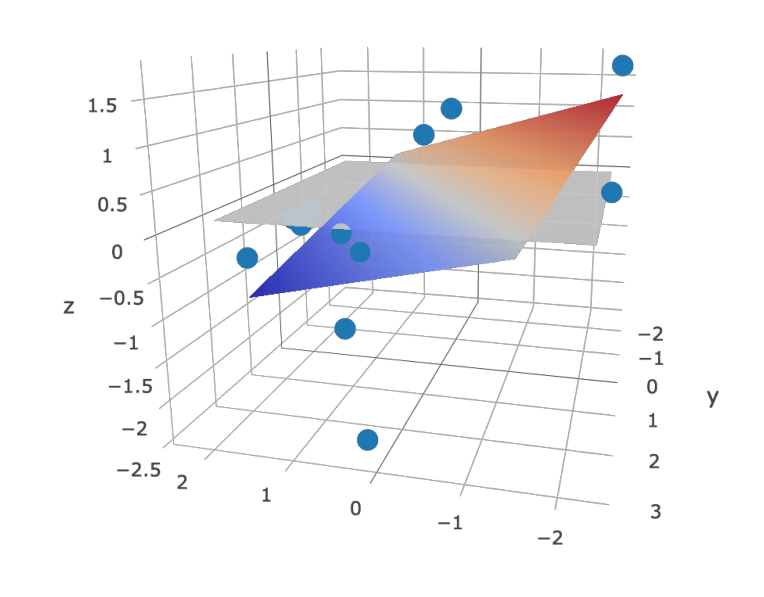
\includegraphics[width=\textwidth]{uncertainty.pdf}
        \caption{}
        \label{fig:MleSubspaceEstimate}
    \end{subfigure}
    ~ %add desired spacing between images, e. g. ~, \quad, \qquad, \hfill etc. 
      %(or a blank line to force the subfigure onto a new line)
    \begin{subfigure}[b]{0.3\textwidth}
        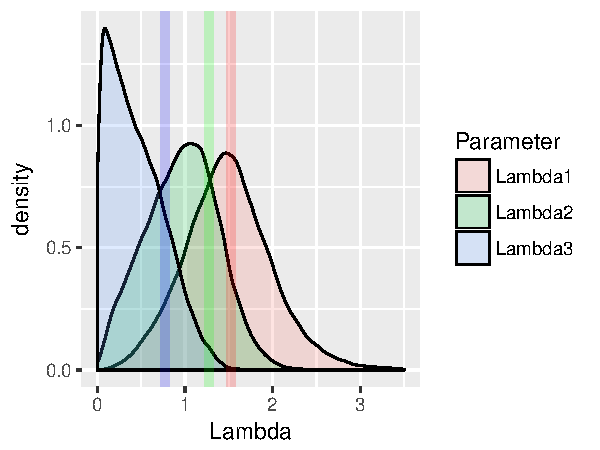
\includegraphics[width=\textwidth]{syntheticLambdaPosterior.pdf}
        \caption{}
        \label{fig:SyntheticPosteriorEstimates}
    \end{subfigure}
    ~ %add desired spacing between images, e. g. ~, \quad, \qquad, \hfill etc. 
    %(or a blank line to force the subfigure onto a new line)
    \begin{subfigure}[b]{0.3\textwidth}
        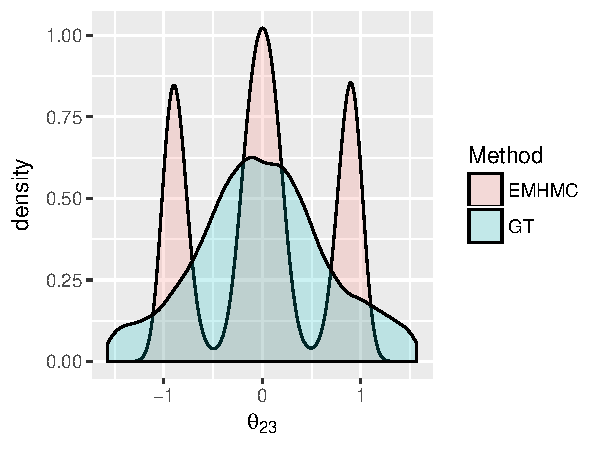
\includegraphics[width=\textwidth]{multiModal.pdf}
        \caption{}
        \label{fig:multiModal}
    \end{subfigure}
    \caption{Inferences for three-dimensional synthetic data. (a) Three-dimensional points, true subspace (grey), and classical PCA point estimate of subspace (colored). (b) Estimated densities from posterior draws of $\Lambda$ parameters A.K.A  the singular values, and point estimates from classical PCA show as colored bars. (c) Avoidance of multi-modal behavior in GT-PPCA versus EMHMC.}\label{fig:synthetic}
\end{figure}

The fully Bayesian approach provided by GT-PPCA in Stan also allows us to examine posterior draws of $\Lambda$ to make probabilistic statements about the inherent dimensionality in our data. Figure \ref{fig:SyntheticPosteriorEstimates} shows estimated densities from posterior draws of $\Lambda$. The posterior of $\Lambda_3$ for example places considerable mass close to zero (58\% of samples were less that 0.5), providing strong evidence that our data is inherently two, not three, dimensional. This is as oppose to classical PCA where we heuristically assess dimensionality based solely on the magnitude of our point estimates.

Lastly, Figure \ref{fig:multiModal} compares posterior samples of our synthetic data from Embedded Manifold HMC (EMHMC) and GT-PPCA in Stan. As explained in section, EMHMC explores the entire Stiefel manifold which includes multiple equivalent modes, where as with GT-PPCA we can eliminate this multi-modal behavior by simply constraining the Givens Transform angle parameters. This is useful both for interpretation and in higher dimensional problems where the number of modes grows exponentially and HMC can not visit all of them. 


%%%%%%%%%%%%%%%%%%%%%%%%%
\subsection{Coagulopathy using hierarchical subspace models}
%%%%%%%%%%%%%%%%%%%%%%%%%
We modeled grouped multi-view hospital data for injured patients using a hierarchical Canonical Correlation Analysis (CCA) model~\citep[chapt.~15.2]{murphy2012machine}. CCA allows to model two types (or views) of data as being a function of two respective latent low dimensional states, but also a common latent state that captures the common information contained in both view. In our case we compared blood protein measurements and clot strength measurements for injured patients belonging to one of four groups depending on the type of injury they had. While the four types of injuries were different enough so that we could not use a single CCA model to capture the characteristics of all models at once, the four groups were not so different as to warrant separate CCA models for each. To share information between the CCA models we placed a hierarchical prior over the orthonormal matrices belonging to the distinct CCA parameters of each group (Figure \ref{fig:CCA}).

\begin{figure}
    \centering
    \begin{subfigure}[b]{0.45\textwidth}
        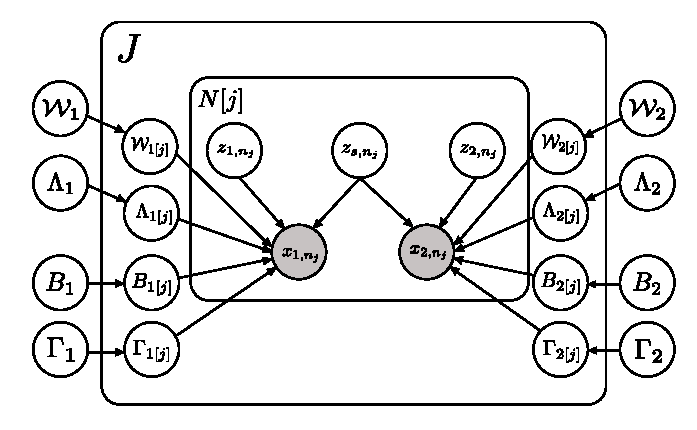
\includegraphics[width=\textwidth]{CCA.pdf}
        \caption{}
        \label{fig:CCA}
    \end{subfigure}
    ~ %add desired spacing between images, e. g. ~, \quad, \qquad, \hfill etc. 
      %(or a blank line to force the subfigure onto a new line)
    \begin{subfigure}[b]{0.45\textwidth}
        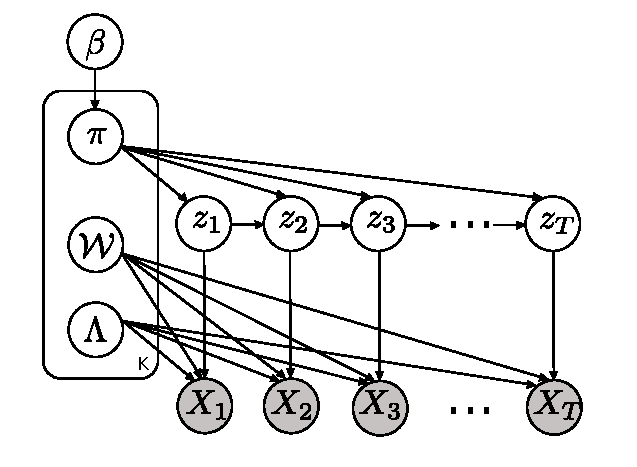
\includegraphics[width=\textwidth]{HMM.pdf}
        \caption{}
        \label{fig:HMM}
    \end{subfigure}
    \caption{Probabilistic graphical models for (a) Hierarchical CCA Model (b) Count Subspace HMM for Network Data.}\label{fig:ccaResults}
\end{figure}

While distributions on the Stiefel manifold such as the Matrix Langevin distribution \citep{muirhead2009aspects} exist, these distributions are difficult to use in practice as computing their density requires evaluating an expensive matrix sum \citep{hoff2009simulation}. By appealing to the Givens Transform and placing a hierarchical prior over the angles of the different orthonormal matrices, we were able to build a hierarchical model over subspaces, a previously intractable task. The hierachical ``shrinks" the posterior median of the orthonormal matrices towards a common mean in addition to reducing the variance of these estimates (Figure \ref{fig:nonHierPosteriors,fig:hierPosteriors}). This is particularly helpful for groups with only a smaller number of observations such as the SW group which only contains 16 patients in comparison of the GSW group with 86 patients. Comparing the angle between the first principal components for the SW and GSW group illustrates how using a hierarchical prior shrinks estimates of subspaces together towards a common hierarchical subspace (Figure \ref{fig:ccaResults}).

\begin{figure}
    \centering
    \begin{subfigure}[b]{0.3\textwidth}
        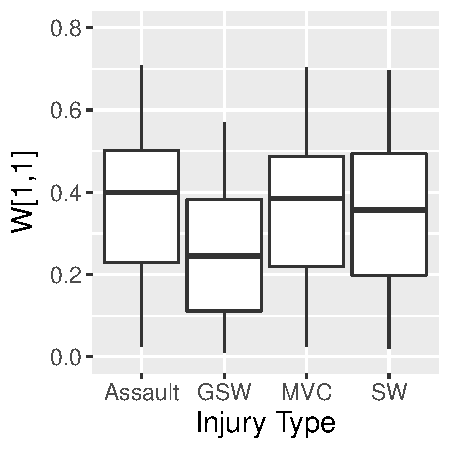
\includegraphics[width=\textwidth]{shrinkageSep.pdf}
        \caption{}
        \label{fig:nonHierPosteriors}
    \end{subfigure}
    ~ %add desired spacing between images, e. g. ~, \quad, \qquad, \hfill etc. 
      %(or a blank line to force the subfigure onto a new line)
    \begin{subfigure}[b]{0.3\textwidth}
        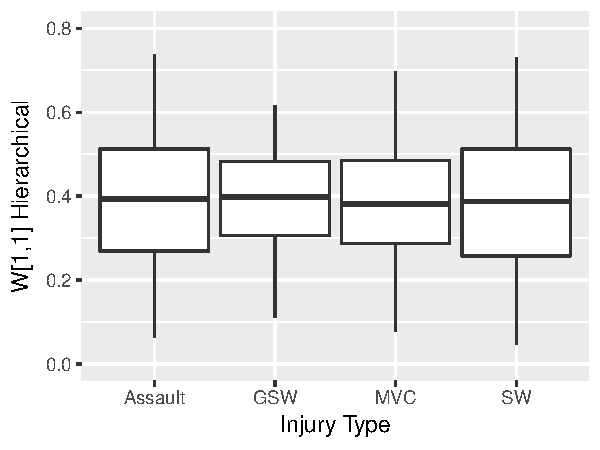
\includegraphics[width=\textwidth]{shrinkageHier.pdf}
        \caption{}
        \label{fig:hierPosteriors}
    \end{subfigure}
    ~ %add desired spacing between images, e. g. ~, \quad, \qquad, \hfill etc. 
    %(or a blank line to force the subfigure onto a new line)
    \begin{subfigure}[b]{0.3\textwidth}
        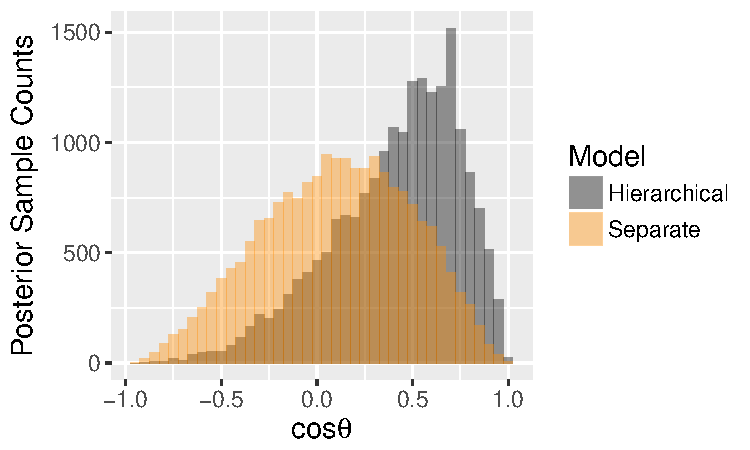
\includegraphics[width=\textwidth]{posteriorCosAngle.pdf}
        \caption{}
        \label{fig:posteriorCosAngle}
    \end{subfigure}
    \caption{Inferences for Hierarchical CCA model.}\label{fig:ccaResults}
\end{figure}

%%%%%%%%%%%%%%%%%%%%%%%%%
\subsection{School Network}
%%%%%%%%%%%%%%%%%%%%%%%%%
We built an HMM subspace for count data to model the hidden time-dependent structure of a network of school children. \citet{stehle2011high} used RF sensors to track the interactions between school children in 12 different classes (two classes for grades 1-6) for an entire school day so as to better understand how disease spreads throughout a network. We collated the number of interactions between each pair of classes in to 10-minute contiguous time windows, giving us 280 symmetric matrices of counts representing the network structure between the different classes throughout the whole day. We modeled the elements of these count matrices as coming from a Poisson distribution whose rate comes from the element-wise exponential of a symmetric matrix$R = \exp (W \Lambda W^T)$, where orthonormal matrix $W$ captures the low-dimensional structure of the network. To model the time varying structure of the network, we posited that the network was always in one of three latent states, that evolve according to a Markov Chain (Figure \ref{fig:HMM}). The three states each have their own associated orthonormal matrix $W_i$ that captures the network structure for that state. 

\begin{figure}
    \centering
    \begin{subfigure}[b]{0.45\textwidth}
        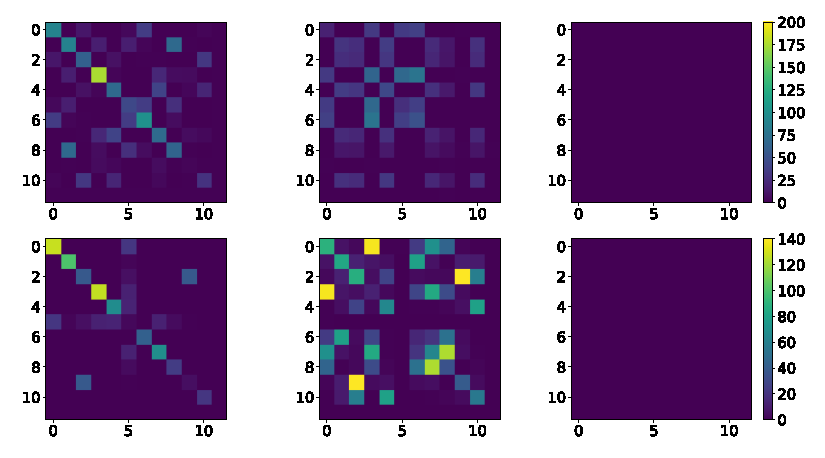
\includegraphics[width=\textwidth]{heatmap.pdf}
        \caption{}
        \label{fig:CCA}
    \end{subfigure}
    ~ %add desired spacing between images, e. g. ~, \quad, \qquad, \hfill etc. 
      %(or a blank line to force the subfigure onto a new line)
    \begin{subfigure}[b]{0.45\textwidth}
        %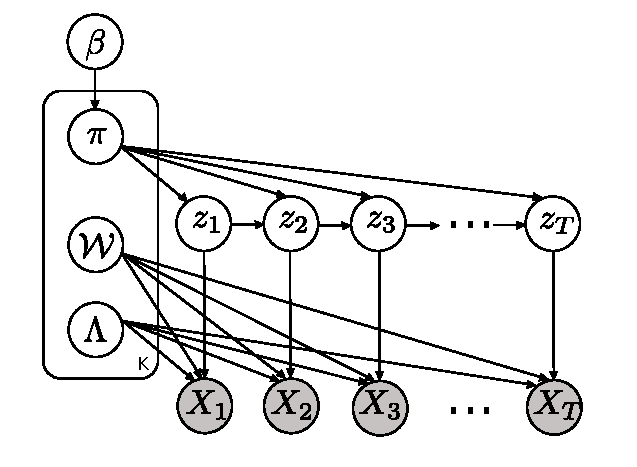
\includegraphics[width=\textwidth]{HMM.pdf}
        \caption{}
        \label{fig:HMM}
    \end{subfigure}
    \caption{Probabilistic graphical models for (a) Hierarchical CCA Model (b) Count Subspace HMM for Network Data.}\label{fig:ccaResults}
\end{figure}

%%%%%%%%%%%%%%%%%%%%%%%%%
%%%%%%%%%%%%%%%%%%%%%%%%%
%%%%%%%%%%%%%%%%%%%%%%%%%
\section{Discussion}
%%%%%%%%%%%%%%%%%%%%%%%%%
%%%%%%%%%%%%%%%%%%%%%%%%%
%%%%%%%%%%%%%%%%%%%%%%%%%
We introduced the Givens Transform as a theoretical representation of orthonormal matrices as well as a practical tool for building complex PPCA-based models in probabilistic programming language like Stan.

\subsubsection*{Acknowledgments}

Use unnumbered third level headings for the acknowledgments. All
acknowledgments go at the end of the paper. Do not include
acknowledgments in the anonymized submission, only in the final paper.

%%%%%%%%%%%%%%%%%%%%%%%%%
%%%%%%%%%%%%%%%%%%%%%%%%%
%%%%%%%%%%%%%%%%%%%%%%%%%
\bibliographystyle{plainnat} % or try abbrvnat or unsrtnat
\bibliography{paperDatabase} % refers to example.bib


\end{document}
